\documentclass[a4paper,12pt]{report}
\usepackage[utf8]{inputenc}
\usepackage[T1]{fontenc}
\usepackage[italian]{babel}
\usepackage{lmodern}
\usepackage{geometry}
\usepackage{enumitem}
\usepackage{graphicx}
\usepackage{setspace}
\usepackage{fancyhdr}
\usepackage{titlesec}
\usepackage{hyperref}
\usepackage{url}
\usepackage{amsmath,amssymb}
\usepackage{listings}
\usepackage{color}
\usepackage{caption}
\usepackage{float}
\usepackage{placeins}

% Geometry for A4 paper with custom margins
\geometry{
  a4paper,
  left=25mm,
  right=25mm,
  top=25mm,
  bottom=25mm,
}

% Hyperref setup
\hypersetup{
  colorlinks=true,
  linkcolor=blue,
  citecolor=blue,
  urlcolor=blue,
  pdftitle={AstroMark-AI - Analisi e Sviluppo},
  pdfauthor={Mario Cosenza, Mario Fasolino, Giulio Sacrestao}
}

\addto\captionsitalian{
\renewcommand{\lstlistingname}{Listato}}

% Header and footer settings
\pagestyle{fancy}
\fancyhf{}
\fancyhead[L]{Pre Processing}
\fancyhead[R]{\nouppercase{\leftmark}}
\fancyfoot[C]{\thepage}

% Title formatting for chapters
\titleformat{\chapter}[display]
  {\normalfont\huge\bfseries}{\chaptertitlename\ \thechapter}{20pt}{\Huge}

% Python code listing configuration
\lstset{
    language=Python,
    basicstyle=\ttfamily\small,
    keywordstyle=\color[RGB]{204,120,50},     % Orange for keywords
    stringstyle=\color[RGB]{6,125,23},        % Dark green for strings
    commentstyle=\color[RGB]{128,128,128},    % Gray for comments
    identifierstyle=\color[RGB]{0,0,0},       % Black for identifiers
    breaklines=true,
    frame=single,
    numbers=left,
    numberstyle=\tiny\color[RGB]{128,128,128},% Tiny gray numbers
    backgroundcolor=\color[RGB]{255,255,255}  % White background
}

% Document title page
\title{%
  \textbf{AstroMark-AI}\\[0.5cm]
  \large Analisi e Sviluppo\\[0.5cm]

  \\
}
\author{%
  Mario Cosenza \and
  Mario Fasolino \and
  Giulio Sacrestao\\[0.5cm]
  Università degli Studi di Salerno\\
  Corso di Fondamenti di Intelligenza Artificiale%
}
\date{Anno Accademico 2024/2025}

\begin{document}

% Cover page with logo
\begin{titlepage}
    \centering
    \vspace*{2cm}
    {\Huge \textbf{AstroMark-AI}}\\[1.5cm]
    {\Large Analisi e Sviluppo}\\[2cm]
    
\includegraphics[width=0.4\textwidth]{images/astromarkLogo.jpg}\\[2cm]
    {\large \textbf{Autori:}}\\[0.5cm]
    Mario Cosenza\\
    Mario Fasolino\\
    Giulio Sacrestao\\[1cm]
    {\small \textbf{Repo:} \url{https://github.com/mariocosenza/astromark-ai}}\\[1cm]
    {\large \textbf{Università degli Studi di Salerno}}\\[0.5cm]
    {\large \textbf{Corso di Fondamenti di Intelligenza Artificiale}}\\[1cm]
    {\large Anno Accademico 2024/2025}
    \vfill
\end{titlepage}

\newpage

% Reset header and footer after the title page
\pagestyle{fancy}
\fancyhf{}
\fancyhead[L]{AstroMark-AI}
\fancyhead[R]{Progetto di NLP}
\fancyfoot[C]{\thepage}

% Table of Contents
\tableofcontents
\newpage

% Include chapters
%! Author = giuliosacrestano
%! Date = 03/02/25

\chapter{Introduzione}

\sloppy
Astromark AI è un'applicazione di machine learning basata su Python, progettata per la classificazione avanzata di testi. Costruita con Flask, espone i suoi servizi tramite endpoint RESTful, facilitando l'integrazione con diversi sistemi. L'applicazione sfrutta moderne tecniche di apprendimento automatico per fornire un'analisi testuale ad alte prestazioni, adatta a compiti come l'analisi del sentiment, la categorizzazione dei contenuti e la classificazione tematica.

\section{Caratteristiche principali}

\begin{itemize}
    \item \textbf{Potenza del Machine Learning}: utilizza algoritmi e modelli avanzati per una classificazione testuale accurata ed efficiente.
    \item \textbf{Integrazione Restful}: offre servizi di classificazione testuale attraverso un'API REST, semplificando l'integrazione in diverse applicazioni.
    \item \textbf{Tecnologia Python e Flask}: sviluppata con Python e Flask, garantisce un'architettura modulare, leggera ed estensibile.
    \item \textbf{Documentazione completa}: include una documentazione dettagliata dell'API per facilitare l'onboarding e l'utilizzo.
\end{itemize}

Astromark AI è la soluzione ideale per sviluppatori e ricercatori alla ricerca di una piattaforma affidabile e di facile utilizzo per la classificazione testuale.
\section{Specifica PEAS}
Di seguito è riportata la descrizione PEAS dell'ambiente operativo di Astromark-AI.
\begin{table}[h]
\centering
\begin{tabular}{|p{4cm}|p{10cm}|}
\hline
\multicolumn{2}{|c|}{\textbf{PEAS}} \\
\hline
\textbf{Performance} & Criteri per valutare il successo dell'agente, ad esempio la percentuale di risposte corrette e utili , il tempo medio di risposta. \\
\hline
\textbf{Environment} & L'ambiente in cui l'agente opera: i ticket inviati, da genitori o docenti, alla Piattaforma Astromark per riceve assistenza su una problematica. \\
\hline
\textbf{Actuators} & I mezzi con cui l'agente agisce sull'ambiente, Astromarl-AI comunicare con l'ambiente organizzando i ticket in base alla categoria. \\
\hline
\textbf{Sensors} & I canali attraverso cui l'agente percepisce l'ambiente, input testuali , nello specifico i ticket . \\
\hline
\end{tabular}
\caption{Specifica PEAS}
\label{tab:peas}
\end{table}

\FloatBarrier

\section{Caratteristiche ambiente}
L'ambiente operativo è:
\begin{itemize}
    \item \textbf{Completamente Osservabile: }possiamo accedere ai ticket in qualsiasi momento
    \item \textbf{Deterministico: }lo stato successivo dell’ambiente è completamente determinato dallo stato corrente e dall’azione eseguita dall’agente
    \item \textbf{Sequenziale: }le scelta dell'azione non dipende dal singolo episodio
    \item \textbf{Statico: }l'ambiente rimane invariato mentre l'agente sta deliberando.
    \item \textbf{Discreto: }l'ambiente fornisce un numero limitato di percezioni
    \item \textbf{Singolo: }l'ambiente consente la presenza di un unico agente.
\end{itemize}


%! Author = giuliosacrestano
%! Date = 03/02/25

\chapter{dataAquisition}
dataAquisition
%! Author = giuliosacrestano
%! Date = 03/02/25

\chapter{textExtractionAndCleanup}
textExtractionAndCleanup
\chapter{Pre Processing}

\section{Introduzione}
La fase di pre-processing approfondisce la trasformazione del testo già estratto e pulito, arricchendo la rappresentazione semantica mediante operazioni quali tokenizzazione, lemmatizzazione e Named Entity Recognition (NER). Queste tecniche avanzate migliorano l'analisi computazionale e preparano il testo per algoritmi di machine learning.

\section{Tokenizzazione, Lemmatizzazione e Named Entity Recognition}
Per incrementare il valore semantico del testo, vengono applicate le seguenti operazioni:
\begin{itemize}
    \item \textbf{Tokenizzazione:} Segmenta il testo in unità minime (token).
    \item \textbf{Lemmatizzazione:} Riduce ogni token alla sua forma base, diminuendo la variabilità morfologica.
    \item \textbf{Named Entity Recognition (NER):} Identifica entità come nomi, organizzazioni e località, etichettandole come ad esempio \texttt{NER\_PERSON}.
\end{itemize}

La seguente funzione integra questi passaggi:

\begin{lstlisting}[language=Python,caption={Funzione process_text}]
def process_text(text):
    cleaned_text = minimal_preprocess(text)
    doc = nlp(cleaned_text)
    tokens = []
    for token in doc:
        if token.is_stop or token.is_punct or token.is_space:
            continue
        lemma = token.lemma_.strip()
        if lemma:
            tokens.append(lemma)
    for ent in doc.ents:
        tokens.append("NER_%s" % ent.label_)
    return ' '.join(tokens)
\end{lstlisting}

\subsection{Deep Learning in spaCy per il Riconoscimento delle Entità}
spaCy impiega modelli basati su deep learning che integrano:
\begin{itemize}
    \item \textbf{Reti Neurali Convoluzionali (CNN):} Per estrarre caratteristiche locali dal testo.
    \item \textbf{Meccanismi di Attenzione:} Per contestualizzare i token in maniera differenziata.
    \item \textbf{Architetture Trasformative:} In grado di modellare relazioni a lungo raggio fra i token.
\end{itemize}
Queste tecnologie permettono di ottenere un elevato livello di accuratezza nel riconoscimento delle entità, anche su testi complessi.

\section{Parallelizzazione del Pre-processing}
Per gestire dataset di grandi dimensioni, la parallelizzazione sfrutta la libreria \texttt{joblib} per distribuire il processo su più core. Il backend "threading" viene utilizzato per ottimizzare l'uso delle risorse hardware. Esempio:

\begin{lstlisting}[language=Python,caption={Funzione parallel\_process\_texts}]
def parallel_process_texts(series, n_jobs=-1):
    logger.info("Parallel text processing with threading backend...")
    with parallel_backend('threading', n_jobs=n_jobs):
        processed = Parallel()(delayed(process_text)(text) for text in series)
    return pd.Series(processed, index=series.index)
\end{lstlisting}
%! Author = giuliosacrestano , mariocosenza
%! Date = 06/02/25

\chapter{Feature Engineering}

\section{Introduzione}
La fase di Feature Engineering è cruciale nel processo di sviluppo di modelli di machine learning, specialmente in ambito Natural Language Processing (NLP). Questa fase si occupa della trasformazione dei dati grezzi in rappresentazioni numeriche che catturino le caratteristiche essenziali dei testi. Un’accurata progettazione in questa fase riduce il rumore e la complessità computazionale, ponendo solide basi per le successive attività di modellazione.

\section{Trasformazione del Testo con TF-IDF}
L'approccio TF-IDF (Term Frequency-Inverse Document Frequency) è una tecnica consolidata per convertire testi in vettori numerici. Essa assegna un peso a ciascun termine in un documento, rendendo più rilevanti i termini discriminanti rispetto a quelli troppo comuni.
Formalmente, il peso \(w(t,d)\) per un termine \(t\) in un documento \(d\) appartenente ad un corpus \(D\) è definito da:
\[
w(t,d) = \text{tf}(t,d) \cdot \log \frac{N}{\text{df}(t)}
\]
Nella quale:
\begin{itemize}
    \item \(\text{tf}(t,d)\) è il conteggio del termine \(t\) nel documento \(d\);
    \item \(N\) rappresenta il numero totale dei documenti nel corpus;
    \item \(\text{df}(t)\) indica il numero di documenti in cui il termine \(t\) appare.
\end{itemize}

I parametri comuni del vettorizzatore TF-IDF sono:
\begin{itemize}
    \item \texttt{use\_idf=True}: attiva la ponderazione inversa.
    \item \texttt{ngram\_range=(1, 2)}: include sia unigrammi che bigrammi per cogliere relazioni tra parole.
    \item \texttt{max\_features=3000}: limita il vocabolario ai termini più rilevanti, migliorando l'efficienza.
    \item \texttt{norm='l2'}: applica la normalizzazione per uniformare i vettori.
    \item \texttt{smooth\_idf=True}: evita problemi di divisione per zero mediante una regolarizzazione dell’IDF.
    \item \texttt{sublinear\_tf=True}: applica una scala logaritmica per attenuare l’effetto di termini dalle frequenze molto elevate.
\end{itemize}

\section{Riduzione della Dimensionalità tramite Truncated SVD}
La rappresentazione TF-IDF genera uno spazio vettoriale di elevata dimensionalità, spesso sparso. La tecnica di Truncated Singular Value Decomposition (SVD) riduce la dimensionalità mantenendo la maggior parte della varianza informativa. Data una matrice \(A \in \mathbb{R}^{m \times n}\) ottenuta dal TF-IDF, la SVD decompone la matrice nel seguente modo:
\[
A = U \Sigma V^T,
\]
Nella quale:
\begin{itemize}
    \item \(U\) e \(V\) sono matrici ortogonali;
    \item \(\Sigma\) è una matrice diagonale con i valori singolari in ordine decrescente.
\end{itemize}
Aplicando la Truncated SVD, si conserva un numero ridotto \(k\) di valori singolari:
\[
A_k = U_k \Sigma_k V_k^T,
\]
con \(k\) scelto in base all'analisi della varianza da preservare (ad esempio, 30, 50, 100). Questa operazione consente di semplificare il modello, eliminando rumore e ridondanze nel set di feature.

\section{Conclusioni}
Una corretta fase di Feature Engineering, tramite TF-IDF e Truncated SVD, permette di ottenere una rappresentazione dei dati testuali efficace e compatta. Tali tecniche riducono il sovrumodello, migliorando le prestazioni computazionali e la generalizzazione del modello di machine learning. Questo approccio formale e ben definito costituisce la base per una modellazione robusta e accurata.
%! Author = giuliosacrestano , mariocosenza
%! Date = 06/02/25

\chapter{Model Building}

\section{Introduzione}
Il processo di \emph{Model Building} è fondamentale per tradurre le rappresentazioni numeriche ottenute in fase di Feature Engineering in un modello capace di classifier testi in modo accurato e robusto. In questo capitolo si descrive formalmente la composizione di una pipeline modulare, l'ottimizzazione degli iperparametri e la scelta del classificatore, fornendo definizioni matematiche ed esempi di implementazione.

\section{Definizione della Pipeline}
La pipeline utilizzata per la modellazione è definita come una funzione composita:
\[
f(x) = f_n \circ f_{n-1} \circ \cdots \circ f_1(x),
\]
dove ciascun \( f_i \) rappresenta una trasformazione applicata al dato grezzo \( x \) (tipicamente un documento testuale). L'output finale \( f(x) \) è la predizione del modello, ossia l'etichetta di classe assegnata.
La pipeline si compone dei seguenti elementi:
\begin{enumerate}
  \item \textbf{Vettorizzazione:} Converte il testo in vettori numerici mediante TF-IDF.
  \item \textbf{(Opzionale) Riduzione della Dimensionalità:} Utilizza tecniche come la Truncated SVD per ridurre lo spazio delle feature, soprattutto se il modello è molto complesso.
  \item \textbf{Classificazione:} Addestra un classificatore, ad esempio \emph{Naive Bayes} o \emph{Support Vector Machine (SVM)}, per assegnare ad ogni documento un'etichetta.
\end{enumerate}

\section{Scelta del Classificatore}
La scelta del classificatore dipende dalla natura dei dati e dalle esigenze del problema:
\begin{itemize}
  \item \textbf{Naive Bayes:} Basato su un modello probabilistico che assume l'indipendenza condizionale delle feature. È particolarmente efficace per dati testuali e regola il proprio comportamento tramite il parametro \texttt{alpha}.
  \item \textbf{Support Vector Machine (SVM):} Utilizza un kernel lineare per individuare l'iperpiano che separa al meglio le diverse classi. L'opzione \texttt{probability=True} permette di stimare probabilità, mentre il parametro \texttt{C} gestisce il compromesso tra margine e errore di classificazione.
\end{itemize}

\section{Implementazione della Pipeline}
Il file seguente (\texttt{build\_pipeline.py}) illustra un esempio completo in Python che definisce la pipeline. Tale file integra la configurazione del vettorizzatore TF-IDF, la possibile applicazione della Truncated SVD e la scelta del classificatore.

\begin{lstlisting}[language=Python,caption={File pipeline.py}]
from typing import Tuple, Dict, Any
from sklearn.pipeline import Pipeline
from sklearn.feature_extraction.text import TfidfVectorizer
from sklearn.decomposition import TruncatedSVD
from sklearn.naive_bayes import MultinomialNB
from sklearn.svm import SVC

class ClassifierType:
    NAIVE_BAYES = 'naive_bayes'
    SVM = 'svm'

def build_pipeline(classifier_type: str) -> Tuple[Pipeline, Dict[str, Any]]:
    # Configurazione del vettorizzatore TF-IDF
    tfidf = TfidfVectorizer(
        use_idf=True,
        ngram_range=(1, 2),
        max_features=3000,
        norm='l2',
        smooth_idf=True,
        sublinear_tf=True
    )

    if classifier_type == ClassifierType.NAIVE_BAYES:
        classifier = MultinomialNB()
        pipeline = Pipeline([
            ('tfidf', tfidf),
            ('clf', classifier)
        ])
        param_grid = {
            'tfidf__min_df': [1, 3],
            'tfidf__max_df': [0.85, 0.90],
            'clf__alpha': [1.0, 1.5, 2.0]
        }
    elif classifier_type == ClassifierType.SVM:
        # In SVM, si applica la Truncated SVD per ridurre la dimensionalità
        svd = TruncatedSVD(n_components=100, random_state=42)
        classifier = SVC(probability=True, kernel='linear', random_state=42)
        pipeline = Pipeline([
            ('tfidf', tfidf),
            ('svd', svd),
            ('clf', classifier)
        ])
        param_grid = {
            'tfidf__min_df': [1, 3],
            'tfidf__max_df': [0.85, 0.90],
            'svd__n_components': [30, 50, 100],
            'clf__C': [0.1, 0.5, 1.0]
        }
    else:
        raise ValueError("Classifier type not supported.")

    return pipeline, param_grid

if __name__ == '__main__':
    # Esempio di utilizzo della pipeline per SVM
    pipeline, params = build_pipeline(ClassifierType.SVM)
    print("Pipeline configurata con i seguenti iperparametri:", params)
\end{lstlisting}

\section{Ottimizzazione degli Iperparametri}
L'ottimizzazione degli iperparametri viene realizzata tramite Grid Search. Formalmente, si cerca:
\[
\theta^* = \arg \min_{\theta \in \Theta} J_{\text{CV}}(\theta),
\]
dove \(J_{\text{CV}}(\theta)\) è il costo medio stimato mediante validazione incrociata (ad esempio, con 5 fold).
Il file seguente (\texttt{run\_grid\_search.py}) mostra un esempio di implementazione della ricerca su griglia per trovare la migliore combinazione di iperparametri.

\begin{lstlisting}[language=Python]
from typing import Tuple, Dict, Any, Optional
import pandas as pd
from sklearn.model_selection import KFold, GridSearchCV
from build_pipeline import build_pipeline, ClassifierType

def run_grid_search(x_data: pd.Series,
                    y_data: pd.Series,
                    classifier_type: str,
                    monitor: bool = False
                   ) -> Tuple[GridSearchCV, Optional[Dict[str, Any]]]:
    pipeline, param_grid = build_pipeline(classifier_type)
    # Suddivisione dei dati in 5 fold per la validazione incrociata
    kf = KFold(n_splits=5, shuffle=True, random_state=42)
    grid_search = GridSearchCV(pipeline, param_grid, cv=kf, n_jobs=-1, verbose=0)

    if monitor:
        # Possibile implementazione del monitoraggio delle risorse (CPU, memoria, tempo)
        pass
    else:
        grid_search.fit(x_data, y_data)

    return grid_search, None

if __name__ == '__main__':
    import numpy as np
    # Esempio con dati sintetici
    x_test = pd.Series(["esempio di testo", "altro esempio", "documento di prova"])
    y_test = pd.Series([0, 1, 0])
    grid, _ = run_grid_search(x_test, y_test, ClassifierType.NAIVE_BAYES)
    print("Miglior configurazione trovata:", grid.best_params_)
\end{lstlisting}

\section{Conclusioni}
Il processo di \emph{Model Building} illustrato in questo documento si basa su una pipeline modulare che integra:
\begin{itemize}
  \item La trasformazione testuale con TF-IDF,
  \item La riduzione della dimensionalità tramite Truncated SVD (quando necessario),
  \item La scelta oculata del classificatore (Naive Bayes o SVM),
  \item e l'ottimizzazione degli iperparametri tramite Grid Search, supportata da validazione incrociata.
\end{itemize}
Questo approccio formale e strutturato garantisce la realizzazione di modelli robusti, efficienti e generalizzabili, in grado di affrontare con successo le sfide poste dalla classificazione testuale.

\chapter{Evaluation}

\section{Introduzione}
In questo capitolo, esamineremo i risultati ottenuti dalla validazione incrociata (\textbf{K-fold cross-validation}) sui modelli di classificazione \textbf{Naive Bayes} e \textbf{Support Vector Machine} (\textbf{SVM}). In particolare, discuteremo delle prestazioni di ciascun modello in termini di accuratezza, matrice di confusione, precisione, recall, F1-score e overfitting. Inoltre, presenteremo un confronto visivo delle metriche per ogni categoria
attraverso grafici a barre. L'obiettivo è confrontare i modelli in modo completo, evidenziando i punti di forza e le debolezze di ciascun approccio.

\section{Metriche di Valutazione dei Modelli}
Per valutare le prestazioni dei modelli, sono state utilizzate le seguenti metriche:

\begin{itemize}
    \item \textbf{Accuratezza}: misura la percentuale di previsioni corrette rispetto al numero totale di previsioni.
    \begin{equation} Accuracy = \frac{TP+TN}{TP+TN+FP+FN}\end{equation}

    \item \textbf{Precisione} (o \textbf{Positive Predictive Value}): indica la percentuale di previsioni positive corrette rispetto a tutte le previsioni positive fatte dal modello.
    \begin{equation} Precision = \frac{TP}{TP+FP}\end{equation}

    \item \textbf{Recall} (o \textbf{Sensibilità} o \textbf{True Positive Rate}): misura la percentuale di veri positivi identificati correttamente dal modello.
    \begin{equation} Recall = \frac{TP}{TP+FN}\end{equation}

    \item \textbf{F1-score}: è la media armonica di precisione e recall, che bilancia entrambi i valori. È utile quando c'è uno squilibrio tra le classi.\begin{equation} F1 = \frac{2*Precision*Recall}{Precision+Recall}\end{equation}
\end{itemize}

\section{Risultati del Modello Naive Bayes}

\subsection{Risultati di Addestramento}

Il modello \textbf{Naive Bayes} ha ottenuto un'accuratezza complessiva del \textbf{92.87\%} sui dati di addestramento. Questa performance suggerisce una buona capacità del modello di generalizzare il comportamento delle classi, mantenendo un buon livello di prestazioni anche su dati non visti. \\ \\
La matrice di confusione, che riporta il numero di previsioni corrette e errate per ciascuna classe, mostra i seguenti risultati:

\begin{figure}[H]
    \centering
    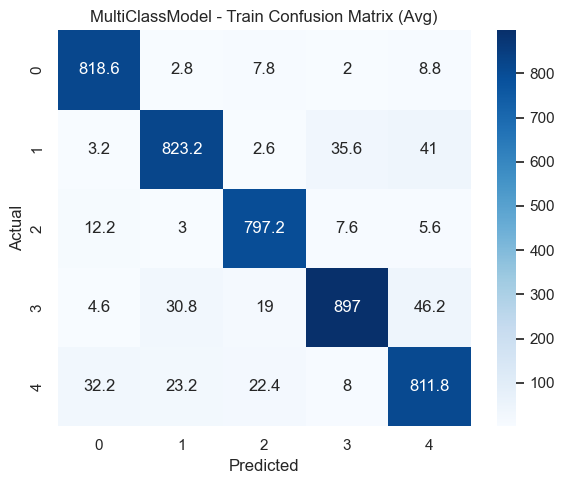
\includegraphics[width=0.8\textwidth]{images/confusion_matrix_train_naive_bayes.png}
    \caption{Matrice di confusione per il training di Naive Bayes}
    \label{fig:confusion_matrix_train_naive_bayes}
\end{figure}

Il modello mostra buone prestazioni complessive, con un'alta percentuale di istanze correttamente classificate, come evidenziato dai valori elevati sulla \textbf{diagonale principale}. Tuttavia, ci sono errori significativi tra alcune classi, in particolare tra le classi 1, 3 e 4, dove il modello ha difficoltà a distinguere correttamente. Questo evidenzia alcune aree in cui il modello potrebbe migliorare nel riconoscere meglio le differenze tra queste classi.   \\ \\
Le metriche per ogni categoria sono mostrate nella seguente tabella e visualizzate nel seguente grafico:

\begin{table}[H]
    \centering
    \begin{tabular}{|c|c|c|c|c|}
        \hline
        \textbf{Categoria} & \textbf{Precision} & \textbf{Recall} & \textbf{F1-score} \\
        \hline
        Accesso & 94.01\% & 97.45\% & 95.70\% \\
        \hline
        Didattica & 93.23\% & 90.90\% & 92.05\% \\
        \hline
        Profilo & 93.90\% & 96.56\% & 95.21\% \\
        \hline
        Segreteria & 94.40\% & 89.91\% & 92.10\% \\
        \hline
        Tecnico & 88.89\% & 90.44\% & 89.65\% \\
        \hline
        media & 93.27\% & 93.28\% & 93.27\% \\
        \hline
        media pesata & 93.16\% & 93.16\% & 93.16\% \\
        \hline
    \end{tabular}
    \caption{Confronto tra precision, recall e F1-score per il training di Naive Bayes}
    \label{tab:metriche_naive_bayes_train}
\end{table}

\begin{figure}[H]
    \centering
    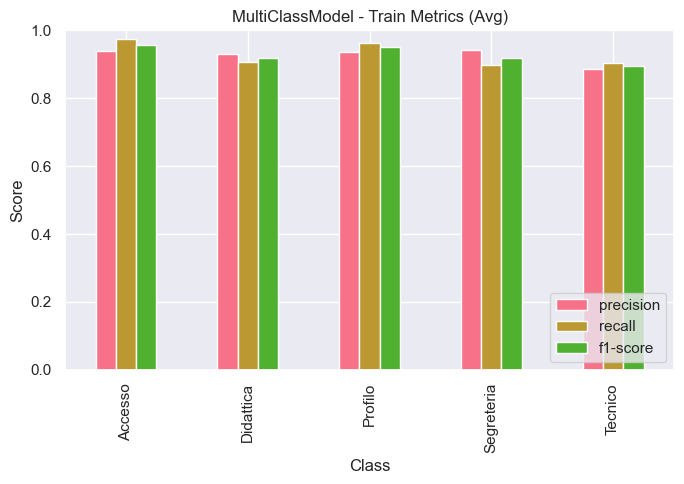
\includegraphics[width=0.8\textwidth]{images/metrics_train_naive_bayes.png}
    \caption{Confronto tra precision, recall e F1-score per il training di Naive Bayes}
    \label{fig:metrics_train_naive_bayes}
\end{figure}

Il modello mostra buone performance complessive, ma nelle categorie \textbf{Segreteria} e \textbf{Tecnico} ci sono margini di miglioramento. \textbf{Segreteria} ha alta precisione ma basso richiamo, mentre \textbf{Tecnico} ha alta capacità di identificare le istanze (buon richiamo), ma con una precisione più bassa. Queste discrepanze suggeriscono che il modello può essere ottimizzato per bilanciare meglio precisione e richiamo in queste categorie.

\subsection{Risultati di Test}

Per quanto riguarda i \textbf{dati di test}, il modello ha ottenuto un'accuratezza del \textbf{89.74\%}, una leggera riduzione rispetto ai dati di addestramento, ma comunque una performance robusta. \\ \\
La matrice di confusione sui dati di test è la seguente:

\begin{figure}[H]
    \centering
    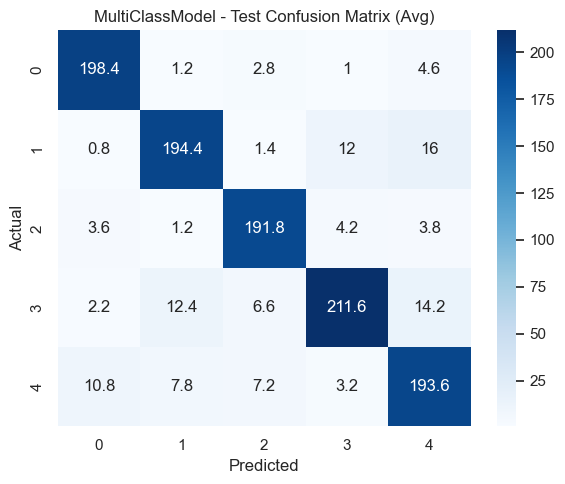
\includegraphics[width=0.8\textwidth]{images/confusion_matrix_test_naive_bayes.png}
    \caption{Matrice di confusione per il testing di Naive Bayes}
    \label{fig:confusion_matrix_test_naive_bayes}
\end{figure}

Mentre le metriche per ogni categoria sono mostrate nella seguente tabella e visualizzate nel seguente grafico:

\begin{table}[H]
    \centering
    \begin{tabular}{|c|c|c|c|c|}
        \hline
        \textbf{Categoria} & \textbf{Precision} & \textbf{Recall} & \textbf{F1-score} \\
        \hline
        Accesso & 91.29\% & 96.01\% & 93.56\% \\
        \hline
        Didattica & 89.92\% & 87.10\% & 88.47\% \\
        \hline
        Profilo & 91.59\% & 94.20\% & 92.87\% \\
        \hline
        Segreteria & 91.33\% & 85.78\% & 88.46\% \\
        \hline
        Tecnico & 84.76\% & 86.88\% & 85.80\% \\
        \hline
        media & 89.78\% & 89.79\% & 89.71\% \\
        \hline
        media pesata & 89.79\% & 89.74\% & 89.71\% \\
        \hline
    \end{tabular}
    \caption{Confronto tra precision, recall e F1-score per il testing di Naive Bayes}
    \label{tab:metriche_naive_bayes_test}
\end{table}

\begin{figure}[H]
    \centering
    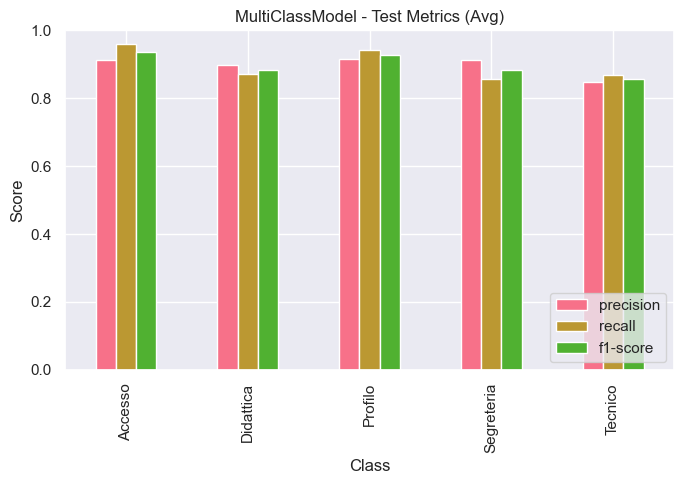
\includegraphics[width=0.8\textwidth]{images/metrics_test_naive_bayes.png}
    \caption{Confronto tra precision, recall e F1-score per il testing di Naive Bayes}
    \label{fig:metrics_test_naive_bayes}
\end{figure}

\subsection{Overfitting}

Per valutare il rischio di \textbf{overfitting}, sono stati analizzati i valori di accuratezza nei diversi fold della validazione incrociata a k-fold. Le differenze tra l'accuratezza dei dati variano tra \textbf{0.02} e \textbf{0.04}, con una media di \textbf{0.0313}. Sebbene vi sia una leggera tendenza all'overfitting, i valori rientrano in un intervallo accettabile, confermando la buona generalizzazione del modello.

\begin{figure}[H]
    \centering
    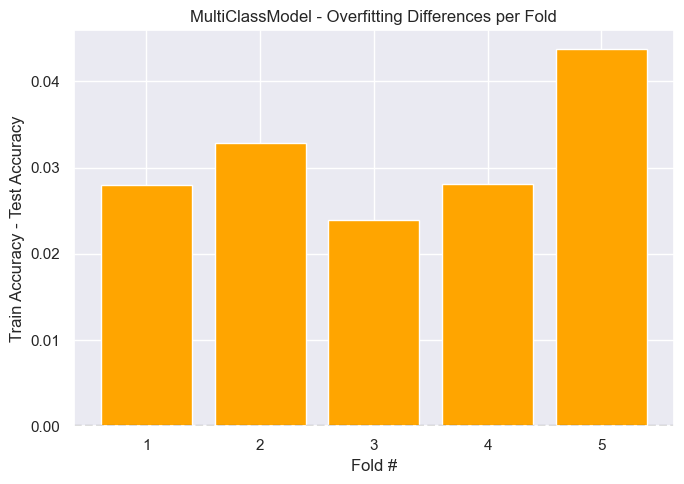
\includegraphics[width=0.8\textwidth]{images/overfitting_naive_bayes.png}
    \caption{Confronto dell'overfitting nei 5 fold per Naive Bayes}
    \label{fig:overfitting_naive_bayes}
\end{figure}

\section{Risultati del Modello Support Vector Machine (SVM)}

\subsection{Risultati di Addestramento}

Il modello \textbf{Support Vector Machine (SVM)} ha ottenuto un'accuratezza complessiva del \textbf{93.17\%} sui dati di addestramento. Questo risultato suggerisce una forte capacità del modello nel generalizzare il comportamento delle classi, mantenendo alte prestazioni anche su dati non visti. \\ \\
La matrice di confusione, che riporta il numero di previsioni corrette ed errate per ciascuna classe, è la seguente:

\begin{figure}[H]
    \centering
    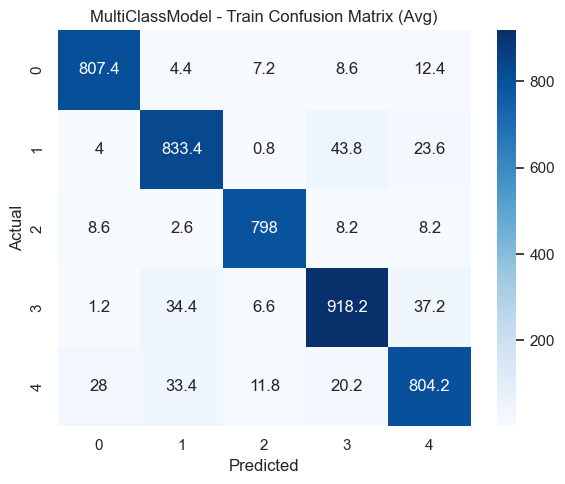
\includegraphics[width=0.8\textwidth]{images/confusion_matrix_train_svm.png}
    \caption{Matrice di confusione per i dati di addestramento con SVM}
    \label{fig:confusion_matrix_train_svm}
\end{figure}

Il modello mostra buone prestazioni complessive, con un’alta percentuale di istanze correttamente classificate, come evidenziato dai valori elevati sulla \textbf{diagonale principale}. Tuttavia, ci sono errori notabili tra alcune classi, in particolare tra le classi 1 e 4, dove il modello fatica a distinguere correttamente. Questo evidenzia alcune aree in cui il modello potrebbe migliorare nel riconoscere meglio le differenze tra queste classi.  \\ \\
Le metriche per ogni categoria sono mostrate nella seguente tabella e visualizzate nel seguente grafico:

\begin{table}[H]
    \centering
    \begin{tabular}{|c|c|c|c|c|}
        \hline
        \textbf{Categoria} & \textbf{Precision} & \textbf{Recall} & \textbf{F1-score} \\
        \hline
        Accesso & 95.08\% & 96.12\% & 95.59\% \\
        \hline
        Didattica & 91.77\% & 92.02\% & 91.89\% \\
        \hline
        Profilo & 96.80\% & 96.65\% & 96.73\% \\
        \hline
        Segreteria & 91.92\% & 92.04\% & 91.98\% \\
        \hline
        Tecnico & 90.82\% & 89.60\% & 90.20\% \\
        \hline
        media & 93.28\% & 93.29\% & 93.28\% \\
        \hline
        media pesata & 93.16\% & 93.17\% & 93.16\% \\
        \hline
    \end{tabular}
    \caption{Confronto tra precision, recall e F1-score per il training di SVM}
    \label{tab:metriche_svm_train}
\end{table}

\begin{figure}[H]
    \centering
    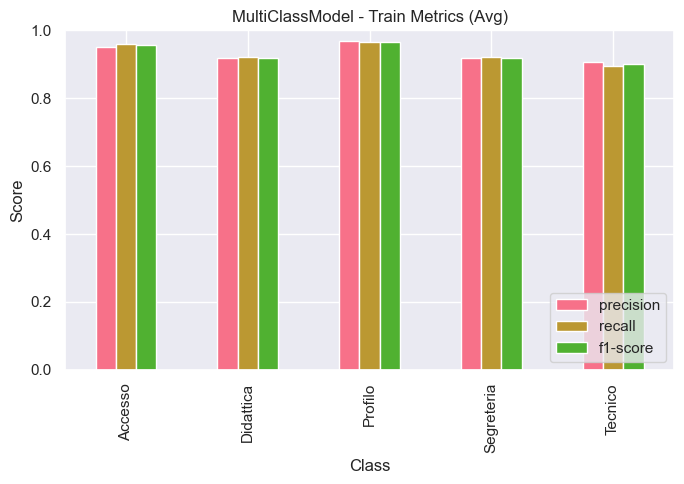
\includegraphics[width=0.8\textwidth]{images/metrics_train_svm.png}
    \caption{Confronto tra precision, recall e F1-score per il training di SVM}
    \label{fig:metrics_train_svm}
\end{figure}

Il modello ha buone performance complessive, ma nelle categorie \textbf{Tecnico} e \textbf{Didattica} ci sono margini di miglioramento. \textbf{Tecnico} mostra un buon richiamo, ma una precisione relativamente bassa, mentre \textbf{Didattica} ha una buona precisione, ma un richiamo leggermente inferiore. Queste discrepanze indicano che il modello potrebbe essere ottimizzato per migliorare l'equilibrio tra precisione e richiamo in queste categorie.

\subsection{Risultati di Test}

Per quanto riguarda i \textbf{dati di test}, il modello ha ottenuto un'accuratezza del \textbf{90.79\%}, con una leggera riduzione rispetto ai dati di addestramento, ma comunque una performance robusta. \\ \\
La matrice di confusione sui dati di test è la seguente:

\begin{figure}[H]
    \centering
    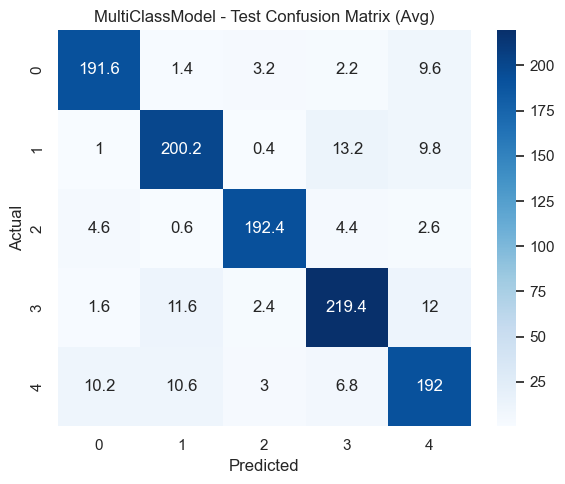
\includegraphics[width=0.8\textwidth]{images/confusion_matrix_test_svm.png}
    \caption{Matrice di confusione per i dati di test con SVM}
    \label{fig:confusion_matrix_test_svm}
\end{figure}

Mentre le metriche per ogni categoria sono mostrate nella seguente tabella e visualizzate nel seguente grafico:

\begin{table}[H]
    \centering
    \begin{tabular}{|c|c|c|c|c|}
        \hline
        \textbf{Categoria} & \textbf{Precision} & \textbf{Recall} & \textbf{F1-score} \\
        \hline
        Accesso & 93.66\% & 95.14\% & 94.37\% \\
        \hline
        Didattica & 88.72\% & 89.42\% & 89.06\% \\
        \hline
        Profilo & 95.89\% & 94.45\% & 95.16\% \\
        \hline
        Segreteria & 88.68\% & 88.82\% & 88.74\% \\
        \hline
        Tecnico & 87.94\% & 86.96\% & 87.43\% \\
        \hline
        media & 90.98\% & 90.96\% & 90.95\% \\
        \hline
        media pesata & 90.81\% & 90.79\% & 90.79\% \\
        \hline
    \end{tabular}
    \caption{Confronto tra precision, recall e F1-score per il testing di SVM}
    \label{tab:metriche_svm_test}
\end{table}

\begin{figure}[H]
    \centering
    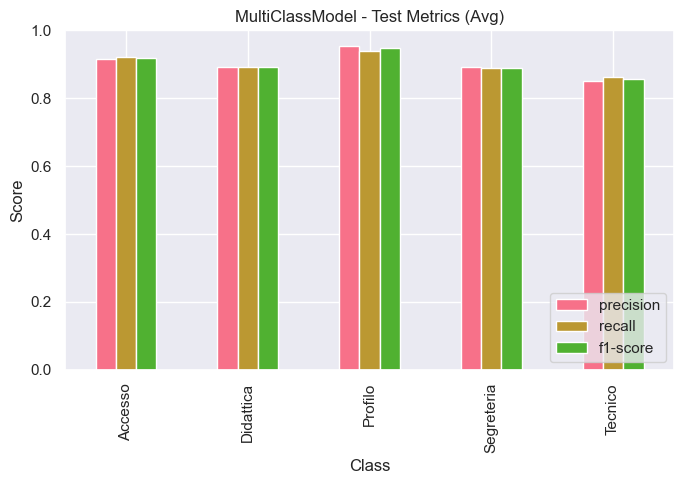
\includegraphics[width=0.8\textwidth]{images/metrics_test_svm.png}
    \caption{Confronto tra precision, recall e F1-score per il testing di SVM}
    \label{fig:metrics_test_svm}
\end{figure}

\subsection{Overfitting}

Per valutare il rischio di \textbf{overfitting}, sono stati analizzati i valori di accuratezza nei diversi fold della validazione incrociata a k-fold. Le differenze tra l'accuratezza dei dati variano tra \textbf{0.02} e \textbf{0.04}, con una media di \textbf{0.0237}. Sebbene ci sia una leggera tendenza all'overfitting, i valori rientrano in un intervallo accettabile, confermando la buona generalizzazione del modello.

\begin{figure}[H]
    \centering
    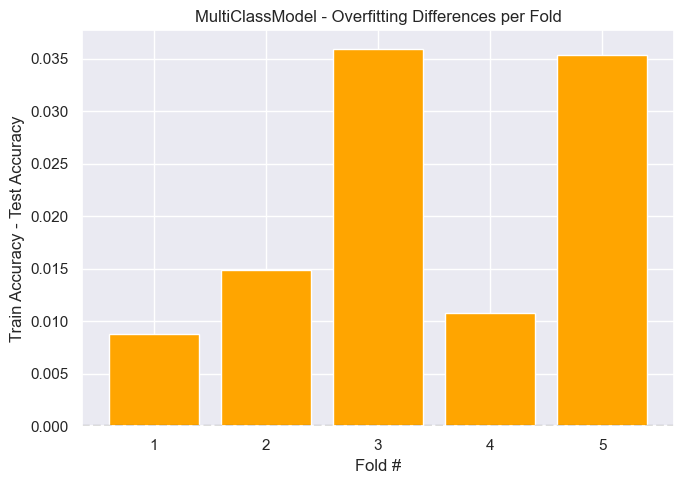
\includegraphics[width=0.8\textwidth]{images/overfitting_svm.png}
    \caption{Confronto dell'overfitting nei 5 fold per SVM}
    \label{fig:overfitting_svm}
\end{figure}

\section{Confronto tra i Modelli}

\subsection{Prestazioni Complessive}

Entrambi i modelli, \textbf{Naive Bayes} e \textbf{SVM}, mostrano prestazioni molto simili. Durante il training, \textbf{Naive Bayes} raggiunge un'accuratezza del 92.87\%, mentre \textbf{SVM} è leggermente migliore con un'accuratezza del 93.17\%. Quando testati sui dati di test, entrambi i modelli registrano una piccola diminuzione delle performance, con \textbf{Naive Bayes} che scende al 89.74\% e \textbf{SVM} che ottiene il 90.79\%. Le metriche di precisione, recall e f1-score sono anch'esse molto simili per entrambi i modelli, suggerendo che entrambi sono abbastanza equilibrati nel bilanciare la capacità di classificare correttamente le istanze e nel ridurre al minimo gli errori.

\begin{table}[H]
    \centering
    \begin{tabular}{|c|c|c|c|c|c|}
        \hline
        \textbf{Modello} & \textbf{Set} & \textbf{Accuracy} & \textbf{Precision} & \textbf{Recall} & \textbf{F1-score} \\
        \hline
        Naive Bayes & Training & 92.87\% & 93.29\% & 92.91\% & 92.88\% \\
        \hline
        Naive Bayes & Test & 89.74\% & 89.91\% & 89.80\% & 89.79\% \\
        \hline
        SVM & Training & 93.17\% & 93.16\% & 93.21\% & 93.16\% \\
        \hline
        SVM & Test & 90.79\% & 90.82\% & 90.85\% & 90.79\% \\
        \hline
    \end{tabular}
    \caption{Confronto tra i modelli in termini di accuracy, precision, recall e F1-score}
    \label{tab:confronto_metriche}
\end{table}


\subsection{Overfitting}

Sia il modello \textbf{Naive Bayes} che il modello \textbf{SVM} mostrano una lieve presenza di \textbf{overfitting}, con differenze tra le performance sui dati che variano tra \textbf{0.02} e \textbf{0.04}. \\ \\
Per meglio visualizzare e comprendere l'andamento dell'overfitting, è stato calcolato il valore della differenza per ogni fold del k-fold cross-validation. La seguente immagine mostra queste differenze per ciascun fold, confrontando l'overfitting tra i modelli Naive Bayes e SVM.

\begin{figure}[H]
    \centering
    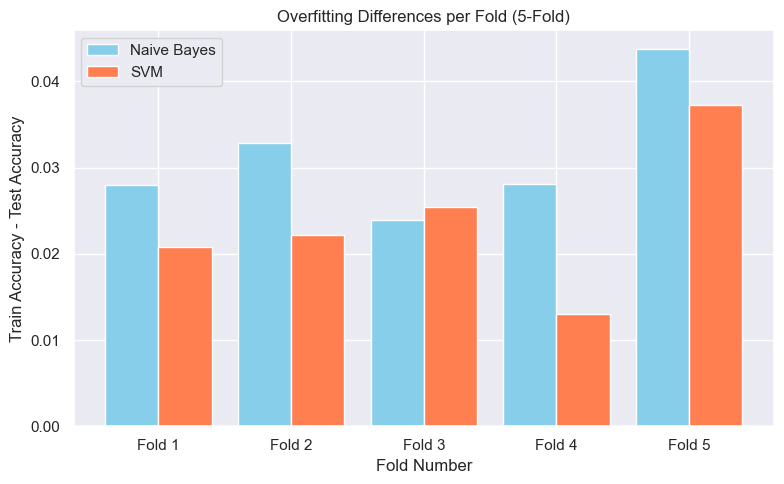
\includegraphics[width=0.8\textwidth]{images/overfitting_differences.png}
    \caption{Confronto dell'overfitting tra Naive Bayes e SVM}
    \label{fig:overfitting_differences}
\end{figure}

\section{Conclusioni}

Entrambi i modelli, Naive Bayes e Support Vector Machine (SVM), hanno mostrato prestazioni eccellenti nel compito di \textbf{classificazione}, evidenziando differenze minime nelle metriche di valutazione. Sebbene il modello SVM ottenga leggermente migliori risultati in termini di accuratezza sui dati di test, con un'accuratezza del \textbf{90.79\%} rispetto al \textbf{89.74\%} di Naive Bayes, la differenza tra i due modelli risulta essere piuttosto contenuta, con un margine di soli pochi punti percentuali. Questo indica che entrambi i modelli sono ben calibrati per il compito e sono capaci di generalizzare efficacemente anche su dati non visti.

\textbf{Naive Bayes}, grazie alla sua semplicità e velocità di esecuzione, potrebbe essere la scelta preferibile in scenari in cui le risorse computazionali sono limitate o in situazioni che richiedono modelli facilmente interpretabili. Inoltre, la capacità di Naive Bayes di gestire efficacemente grandi volumi di dati con risorse relativamente basse lo rende adatto per applicazioni in tempo reale o su dispositivi con risorse limitate.

D'altra parte, il modello \textbf{SVM} si distingue per una maggiore precisione in alcuni casi, come evidenziato dalle metriche di precisione e recall, ed è generalmente considerato una scelta solida quando è necessaria una maggiore accuratezza, specialmente in contesti dove la performance sui dati di test è cruciale e si dispone di risorse computazionali adeguate. SVM è inoltre più adatto per situazioni che richiedono una maggiore capacità di generalizzazione rispetto a modelli con assunzioni più forti, come Naive Bayes.

In definitiva, entrambi i modelli sono validi per il problema in esame e presentano un buon compromesso tra \textbf{accuratezza} e capacità di \textbf{generalizzazione}. La scelta finale tra Naive Bayes e SVM dipenderà da considerazioni specifiche relative all'ambiente applicativo, come la disponibilità di risorse computazionali, la necessità di interpretabilità del modello e la priorità data a una leggera miglioria nelle prestazioni rispetto alla velocità di esecuzione.





\chapter{Deployment}
\newtheorem{definition}{Definizione}[chapter]

\section{Server di Sviluppo Flask}
Flask fornisce un server di sviluppo integrato che facilita il testing e lo sviluppo dell'applicazione. Il server viene configurato nel file principale dell'applicazione attraverso una semplice istruzione che ne definisce le modalità di esecuzione:

\begin{lstlisting}[language=Python, caption=Configurazione Server Flask]
if __name__ == '__main__':
    app.run(debug=True)
\end{lstlisting}

\begin{definition}[Server di Sviluppo]
Il server di sviluppo Flask è un web server leggero integrato nel framework, progettato per facilitare il processo di sviluppo e debug dell'applicazione. Non è ottimizzato per l'ambiente di produzione e non dovrebbe essere utilizzato in tale contesto.
\end{definition}

\section{Endpoints dell'API}
L'applicazione espone due endpoint principali per i servizi basati su intelligenza artificiale. Il primo endpoint gestisce l'orientamento degli studenti attraverso il modello Gemini di Google, mentre il secondo si occupa della classificazione dei ticket di supporto.
\begin{definition}[Endpoint]
Un endpoint rappresenta un punto di accesso specifico dell'API che risponde a determinate richieste HTTP. Nel contesto di questa applicazione, gli endpoint sono progettati per gestire richieste POST e restituire risposte in formato testuale con codifica UTF-8.
\end{definition}

\section{Integrazione con Spring}
L'applicazione Spring si interfaccia con il servizio Flask utilizzando RestTemplate per le comunicazioni HTTP. Questa integrazione permette di mantenere una separazione dei contesti applicativi garantendo al contempo una comunicazione efficiente tra i servizi.

\begin{lstlisting}[language=Java, caption=Codice Integrazione Spring]
private String callTicketService(String title, String message) {
    var restTemplate = new RestTemplate();
    var formData = new LinkedMultiValueMap<String, String>();
    formData.add("title", title);
    formData.add("message", message);
    
    var headers = new HttpHeaders();
    headers.setContentType(
        MediaType.APPLICATION_FORM_URLENCODED);
    
    var requestEntity = new HttpEntity<MultiValueMap<String, String>>(
        formData, headers);
    
    ResponseEntity<String> response = restTemplate.postForEntity(
        ticketServiceUrl, 
        requestEntity, 
        String.class);
    
    return response.getBody();
}
\end{lstlisting}

\begin{definition}[RestTemplate]
RestTemplate è una classe fornita da Spring Framework che semplifica l'interazione con servizi REST. Gestisce automaticamente la serializzazione e deserializzazione degli oggetti Java in richieste HTTP e viceversa.
\end{definition}

\section{Configurazione}
La configurazione dell'applicazione Flask include alcuni parametri fondamentali per il corretto funzionamento del servizio. In particolare, viene gestita la codifica JSON per supportare caratteri UTF-8 e viene configurato il sistema di logging per il monitoraggio dell'applicazione:

\begin{lstlisting}[language=Python, caption=Configurazione Base]
app.config['JSON_AS_ASCII'] = False

logging.basicConfig(
    level=logging.INFO,
    format='[%(levelname)s] %(message)s'
)
\end{lstlisting}

Le variabili d'ambiente necessarie includono la chiave API per il servizio Gemini e l'URL del servizio ticket in Spring. Queste configurazioni devono essere gestite in modo appropriato nell'ambiente di deployment per garantire il corretto funzionamento dell'applicazione.
\chapter{Conclusioni Finali}
L'analisi e lo sviluppo di \textit{AstroMark-AI} hanno evidenziato l'efficacia dell'approccio adottato per la classificazione testuale mediante tecniche di machine learning. Il confronto tra i modelli \textit{Naive Bayes} e \textit{Support Vector Machine (SVM)} ha mostrato prestazioni simili, con \textit{SVM} che ha ottenuto un leggero vantaggio in termini di accuratezza, raggiungendo il $85.95\%$ rispetto all'$88.92\%$ di \textit{Naive Bayes}. Tuttavia, entrambi i modelli hanno dimostrato una buona generalizzazione e robustezza.

L'uso di \textit{TF-IDF} come metodo di rappresentazione testuale si è rivelato efficace per l'elaborazione dei dati, garantendo un equilibrio tra interpretabilità e prestazioni computazionali. La pipeline di preprocessing e feature engineering ha permesso di migliorare la qualità dei dati, riducendo il rumore e ottimizzando la rappresentazione delle informazioni.

Dal punto di vista pratico, \textit{Naive Bayes} si conferma una scelta ideale per applicazioni che richiedono rapidità di esecuzione e basso consumo di risorse, mentre \textit{SVM} è preferibile nei casi in cui è necessaria una maggiore precisione. La decisione su quale modello adottare dipenderà quindi dal contesto applicativo e dai vincoli computazionali.

Infine, l'implementazione e il deployment del sistema su un'architettura basata su \textit{Flask} e la sua integrazione con \textit{Spring} hanno dimostrato la fattibilità di un sistema scalabile ed efficiente. Questo lavoro costituisce una base solida per futuri miglioramenti, tra cui l'esplorazione di modelli neurali più avanzati o l'integrazione di tecniche di apprendimento attivo per migliorare continuamente le prestazioni del sistema.

\subsection{Limitazioni}
Un aspetto critico di questo lavoro è la validazione delle performance utilizzando un dataset generato artificialmente tramite modelli di \textit{Large Language Models} (LLM) piuttosto che dati raccolti da scenari d’uso reali. Questo introduce alcune limitazioni significative:

\begin{itemize}
    \item \textbf{Mancanza di variabilità naturale}: i dati generati tendono a presentare una struttura e una distribuzione più regolari rispetto a quelli raccolti da utenti reali, riducendo la capacità del modello di adattarsi a espressioni linguistiche spontanee e meno formali.
    \item \textbf{Possibili bias nei dati sintetici}: poiché i dati sono generati da AI pre-addestrate su fonti specifiche, potrebbero riflettere le limitazioni intrinseche dei modelli linguistici, trasmettendo eventuali pregiudizi o schemi linguistici artificiali che non rispecchiano perfettamente l'uso effettivo del linguaggio.
    \item \textbf{Difficoltà nella generalizzazione}: un modello addestrato su dati sintetici potrebbe ottenere buone prestazioni sul dataset di test, ma riscontrare difficoltà significative quando applicato su dati provenienti da un ambiente reale, dove il linguaggio può essere più variegato e meno strutturato.
    \item \textbf{Assenza di rumore tipico delle interazioni reali}: nei dati reali sono presenti errori grammaticali, abbreviazioni, linguaggio informale e altre variabili che un dataset generato artificialmente non sempre cattura in modo fedele.
\end{itemize}

\subsection{Lavori futuri}
Per superare queste limitazioni e rendere il modello più robusto in contesti reali, alcune possibili direzioni future includono:
\begin{itemize}
    \item L'adozione di modelli basati su reti neurali per migliorare la capacità di generalizzazione.
    \item L'integrazione di un sistema di \textit{active learning} per affinare il modello con nuovi dati etichettati in modo incrementale.
    \item La raccolta e l'annotazione di dati reali per migliorare la qualità del dataset e confrontare le performance con dati sintetici.
    \item L'ottimizzazione delle prestazioni attraverso tecniche di compressione dei modelli e accelerazione hardware.
\end{itemize}

Con queste prospettive, \textit{AstroMark-AI} si pone come una piattaforma versatile e in continua evoluzione, pronta a rispondere alle esigenze di analisi automatizzata del testo con strumenti di intelligenza artificiale.


\appendix
\chapter{Modelli Generativi e l'Orientamento Universitario}
\subsection*{Premessa}
La presente appendice approfondisce due tematiche di rilevanza nel contesto educativo: l'impiego di modelli generativi e la problematica dell'orientamento universitario. Quest'ultimo aspetto è particolarmente cruciale per gli studenti di scuola secondaria di secondo grado, che devono confrontarsi con un panorama educativo complesso e in continua evoluzione.

\subsection*{Il Problema dell'Orientamento Universitario}
L'orientamento universitario comporta diverse sfide:
\begin{itemize}
    \item \textbf{Scelta del percorso di studi:} valutare le proprie attitudini, interessi e performance scolastiche per identificare il corso di studi più adatto.
    \item \textbf{Informazione e supporto:} la mancanza di un riferimento strutturato può rendere difficoltosa la scelta, lasciando gli studenti senza un adeguato sostegno informativo.
    \item \textbf{Adattamento al mercato del lavoro:} in un contesto in rapida evoluzione, la decisione sul percorso formativo deve tener conto anche delle future opportunità professionali.
\end{itemize}
L’utilizzo dei modelli generativi offre l’opportunità di supportare il processo decisionale, fornendo analisi approfondite basate sui dati individuali e sulle tendenze del mercato, contribuendo a orientamenti più informati e personalizzati.

\subsection*{Modelli Generativi e la loro Configurazione}
I modelli generativi utilizzano algoritmi di intelligenza artificiale per creare contenuti testuali partendo da un input specifico. La configurazione del modello si basa su parametri chiave:
\begin{itemize}
    \item \textbf{Temperature:} controlla il grado di casualità e creatività dell'output. Valori alti generano risultati più variabili.
    \item \textbf{Top\_p e Top\_k:} limitano il ventaglio delle possibili scelte durante la generazione, indirizzando il modello verso risposte più coerenti.
    \item \textbf{Max\_output\_tokens:} definisce il numero massimo di token, ovvero le unità base del testo, che il modello può produrre.
\end{itemize}
La gestione delle chiavi API avviene tramite variabile d'ambiente, per garantire l’accesso protetto ai servizi di intelligenza artificiale.

\subsection*{Esempio di Codice}
Di seguito viene riportato un esempio in Python che illustra come configurare e utilizzare un modello generativo per fornire suggerimenti formali sull'orientamento universitario:

\begin{lstlisting}[language=Python, caption=Esempio di utilizzo di un modello generativo per l'orientamento universitario, basicstyle=\ttfamily\small, breaklines=true]
import os
import google.generativeai as genai

# Configurazione dei parametri del modello generativo
config = genai.types.GenerationConfig(
    temperature=1.5,  # Regola la creativita del testo
    top_p=0.7,        # Limita il ventaglio delle scelte possibili
    top_k=1,          # Seleziona la scelta piu probabile
    max_output_tokens=100  # Limite massimo per la lunghezza del testo generato
)

def genera_suggerimenti(voti):
    # Configurazione del client con la chiave API sicura
    genai.configure(api_key=os.environ.get("GEMINI_API_KEY"))
    modello = genai.GenerativeModel("gemini-1.5-flash", generation_config=config)

    # Definizione del prompt per la richiesta di orientamento
    prompt = f"Fornisci un consiglio formale per l'orientamento universitario. Voti: {voti}"
    risposta = modello.generate_content(prompt)
    return risposta.text
\end{lstlisting}
\end{document}